\documentclass{article}
% Package and macro definitions for CSC 503
% Originally prepared August 23, 2012 by Jon Doyle

%%% Page dimensions
\setlength{\oddsidemargin}{0in}
\setlength{\evensidemargin}{0in}
\setlength{\topmargin}{0in}
\setlength{\textheight}{9in}
\setlength{\textwidth}{6.5in}
\setlength{\headheight}{0in}
\setlength{\headsep}{0in}
\setlength{\footskip}{0.5in}

%%% Font and symbol definition packages
\usepackage{times} 
\usepackage{helvet} 
\usepackage{alltt}
\usepackage{amsfonts, amsmath}
\usepackage{amssymb}

%%% The modified Sellinger fitch.sty file
\input{fitchhr.sty}

\newcommand{\Z}{\mathbb{Z}}
\newcommand{\Q}{\mathbb{Q}}
\newcommand{\R}{\mathbb{R}}
\newcommand{\N}{\mathbb{N}}
\def\land{\wedge}
\def\lor{\vee}
\def\implies{\rightarrow}
\def\iff{\leftrightarrow}
\def\turn{\vdash}
\def\Cn{\text{Cn}}
\def\Th{\text{Th}}
\def\defeq{\stackrel{\rm def}{=}}

%%% The environment for providing answers to problems
\newenvironment{answer}%
{\par\noindent\textbf{Answer}\par\noindent}%
{}


\usepackage{amsfonts, amsmath, amsthm}
\usepackage{tikz}
\usetikzlibrary{arrows,automata}

\def\Sometime{\mathord{\mathsf{F}}}
\def\Forever{\mathord{\mathsf{G}}}
\def\Next{\mathord{\mathsf{O}}}
\def\NextX{\mathord{\mathsf{X}}}
\def\Until{\mathrel{\mathsf{U}}}
\def\Release{\mathrel{\mathsf{R}}}
\def\WeakUntil{\mathrel{\mathsf{W}}}
\def\Before{\mathrel{\mathsf{B}}}
\def\True{\mathord{\mathsf{true}}}
\def\All{\mathord{\mathsf{A}}}
\def\Exists{\mathord{\mathsf{E}}}
\def\Every{\mathord{\mathsf{E}}}

\title{CSC 503 Homework Assignment 9}
\author{Due October 29, 2014}
\date{October 22, 2014}

\begin{document}
\maketitle

\begin{itemize}
\item \textbf{[40 points total]} Consider the transition model ${\cal
    M}_2$ depicted in Figure \ref{f2} in answering the following
  questions about LTL and CTL statements.
  \begin{figure}[h]
    \centering
    \caption{Model ${\cal M}_2$}
\begin{center}

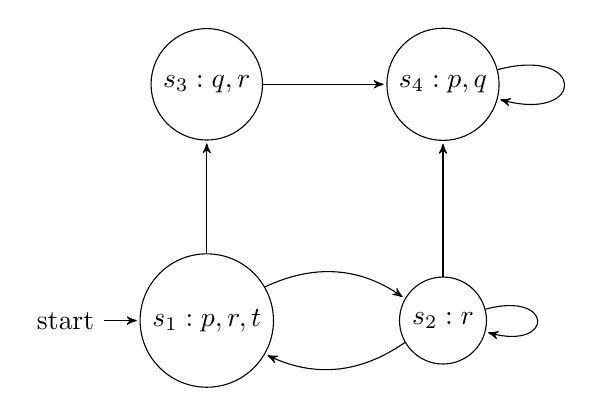
\begin{tikzpicture}[>=stealth',shorten >=1pt,auto,node distance=3cm]
  \node[state] (q3)      {$s_3: q,r$};
  \node[state] (q4)    [right of=q3] {$s_4: p,q$};
  \node[initial,state] (q1)   [below of=q3]   {$s_1: p,r,t$};
  \node[state] (q2)   [right of=q1]   {$s_2: r$};

  \path[->] 
        (q3) edge         node {} (q4)
        (q4) edge [loop right] node {} (q4)
        (q1) edge         node {} (q3)
        (q2) edge         node {} (q4)
        (q2) edge [loop right] node {} (q2)
        (q1) edge    [bend left] node {} (q2)
        (q2) edge    [bend left] node {} (q1);
\end{tikzpicture}
\end{center}
\label{f2}
\end{figure}
  \begin{enumerate}
  \item \textbf{[8 points]} Does ${\cal M}_2, s_4 \models r \implies
    q$?  Explain why or why not.
    \begin{answer}
    	${\cal M}_2, s_4 \models r \implies q$ is True. \newline
    	\textbf{Explanation}: In the state $s_4$, $r$ is false and then the
    	implication is always true. So according to the definition this holds.
    \end{answer}
    \bigskip
  \item \textbf{[8 points]} Does ${\cal M}_2, s_1 \models r \implies
    q$?  Explain why or why not.
    \begin{answer}
    	${\cal M}_2, s_1 \models r \implies q$ is False. \newline
    	\textbf{Explanation}: In the state $s_1$ in the model, $r$ is true. Thus
    	for the implication to be true $q$ also needs to be true in state $s_1$,
    	which is not the case. Hence this does not hold.
    \end{answer}
    \bigskip
  \item \textbf{[8 points]} Does ${\cal M}_2, s_3 \models \Sometime
    \neg t$?  Explain why or why not.
    \begin{answer}
    	${\cal M}_2, s_3 \models \Sometime \neg t$ is True. \newline
    	\textbf{Explanation}: The Model starting from state $s_3$ contains only one
    	path which is $s_3-(s_4)$. In both the state $neg t$ is true since $t$ is
    	false. Thus $\Sometime \neg t$ is true since it occurs atleast once in the
    	path.
    \end{answer}
    \newpage
  \item \textbf{[8 points]} Does ${\cal M}_2, s_1 \models \Sometime
    \neg t$?  Explain why or why not.
    \begin{answer}
    	${\cal M}_2, s_1 \models \Sometime \neg t$ is True. \newline
    	\textbf{Explanation}: $t$ is only true in state $s_1$. Hence $\neg t$ is
    	false in state $s_1$ only. All the paths starting at state $s_1$ have
    	atleast one transition to states $s_2$ or $s_3$ and thus atleast once
    	$\neg t$ is true. Thus overall for all paths from state $s_1$ $\Sometime
    	\neg t$ is also true.
    \end{answer}
    \bigskip
  \item \textbf{[8 points]} Does ${\cal M}_2, s_2 \models \neg \Exists
    \Forever r$?  Explain why or why not.
    \begin{answer}
    	${\cal M}_2, s_2 \models \neg \Exists \Forever r$ is False. \newline
    	\textbf{Explanation}: The formula means that there exists no path where
    	$\Forever r$ is true. Now consider a path $(s_2)$, which is looping through
    	$s_2$ till infinity. In this path $r$ is always true. Thus $\Forever r$ is
    	also true. And since we found atleast one path starting from $s_2$ where
    	$r$ is always true, so $\Exists \Forever r$ is also true, which means that
    	the given expression is False since its a complementary formula to
    	$\Exists \Forever r$.
    \end{answer}
    \bigskip
  \item \textbf{[8 points]} Does ${\cal M}_2, s_4 \models \neg \Exists
    \Forever r$?  Explain why or why not.
    \begin{answer}
    	${\cal M}_2, s_4 \models \neg \Exists \Forever r$ is True.	\newline
    	\textbf{Explanation}: The model contains only a single path from starting
    	from $s_4$ which is $(s_4)$. The expression $\neg \Exists \Forever r$ can
    	also be represented as $\All \Sometime \neg r$. The first formula means
    	that there doesn't exists any path for which $r$ is always true and if we
    	take the negative sign inside then we get the second formula which means
    	for all paths $\neg r$ exists sometime in the future. Now in the path
    	$(s_4)$ which is the only one in the model starting with state $s_4$ has
    	$\neg r$ as true since $r$ is false. Thus $\Sometime \neg r$ is also true
    	and since its the only path so $\All \Sometime \neg r$ is also true. Thus
    	$\neg \Exists \Forever r$ is also true since both are the same.
    \end{answer}
    \bigskip
  \item \textbf{[8 points]} Does ${\cal M}_2, s_3 \models \Exists
    \Sometime q$?  Explain why or why not.
    \begin{answer}
    	${\cal M}_2, s_3 \models \Exists \Sometime q$ is True.	\newline
    	\textbf{Explanation}: Model starting from $s_3$ has only one path which is
    	$s_3-(s_4)$. In this path we can see that $q$ is true in state $s_3$ as
    	well as $s_4$ on the path. Thus $\Exists \Sometime q$ is true.
    \end{answer}
    \bigskip
  \item \textbf{[8 points]} Does ${\cal M}_2, s_1 \models \Exists
    \Sometime q$?  Explain why or why not.
    \begin{answer}
    	${\cal M}_2, s_1 \models \Exists \Sometime q$ is True.	\newline	
    	\textbf{Explanation}: The formula $\Exists \Sometime q$ means that there
    	exists atleast one path where $\Sometime q$ is true. Consider a path
    	$s_1-s_3-(s_4)$ which is one of the path in the Model. In this path $q$ is
    	true in state $s_3$ as well as $s_4$. Thus $\Sometime q$ is also true. And
    	since we found one path where $\Sometime q$ is true, thus $\Exists
    	\Sometime q$ is also true.
    \end{answer}
    \bigskip
  \item \textbf{[8 points]} Does ${\cal M}_2, s_4 \models \All
    \NextX \All \Forever (p \lor q)$?  Explain why or why not.
    \begin{answer}
    	${\cal M}_2, s_4 \models \All \NextX \All \Forever (p \lor q)$ is True.
    	\newline
    	\textbf{Explanation}: The formula $\All \NextX \All \Forever (p \lor q)$
    	means that the formula $\All \Forever (p \lor q)$ is true next on all
    	paths. In the model starting from state $s_4$ there is only one path
    	$(s_4)$. On this path $(p \lor q)$ is always true starting from the second
    	node which is again $s_4$. Thus $\All \NextX \All \Forever (p \lor q)$ is
    	true as there is only one path and the formula holds in that path.
    \end{answer}
    \bigskip
  \item \textbf{[8 points]} Does ${\cal M}_2, s_2 \models \All \NextX
    \All \Forever (p \lor q)$?  Explain why or why not.
    \begin{answer}
    	${\cal M}_2, s_2 \models \All \NextX \All \Forever (p \lor q)$ is False.
    	\newline
    	\textbf{Explanation}: The formula $\All \NextX \All \Forever (p \lor q)$
    	means that the formula $\All \Forever (p \lor q)$ is true next on all
    	paths. Consider one of the paths as $(s_2)$, which is looping through state
    	$s_2$. In this path neither $p$ nor $q$ is ever true. Thus we know that for
    	this particular path violates the formula. Hence $\All \NextX \All
    	\Forever (p \lor q)$ is false.
     \end{answer}
    \bigskip
  \end{enumerate}

%\newpage

\item \textbf{[20 points]} List all subformulas of the CTL formula,
  using Convention 3.13 (p.\ 209) to resolve ambiguities.
  \begin{displaymath}
    \Exists [\All \NextX p \Until (\neg \Exists \NextX q \land \All
    [\neg p \Until \All \Forever (p \lor q)])]
  \end{displaymath}
\end{itemize}
	\begin{answer}
	The subformula of the given formula is as follows:-
		\begin{enumerate}
		  \item $\Exists [\All \NextX p \Until (\neg \Exists \NextX q \land \All [\neg
		  p \Until \All \Forever (p \lor q)])]$
		  \item $\All \NextX p$
		  \item $p$
		  \item $\neg \Exists \NextX q \land \All [\neg p \Until \All \Forever (p \lor
		  q)]$
		  \item $\neg \Exists \NextX q$
		  \item $\Exists \NextX q$
		  \item $q$
		  \item $\All [\neg p \Until \All \Forever (p \lor q)]$
		  \item $\neg p$
		  \item $\All \Forever (p \lor q)$
		  \item $p \lor q$
		\end{enumerate}
	\end{answer}
\end{document}
